\newpage
\onecolumn
\section{Kinematica van een Punt}
\label{sec:KinematicaPunt}


\subsection{Baan van een Punt}
\label{sec:BaanPunt}
\[
  \vec{r} = \vec{r}\left( t \right) =
  \left\{
        \begin{array}[h]{lcr}
	       x & = & x\left( t \right)\\
	       y & = & y\left( t \right)\\
	       y & = & y\left( t \right)\\
        \end{array}
  \right.
\]

\paragraph{Elementaire Booglengte}
\label{sec:ElementaireBooglengte}
\[
  \d{s} = \sqrt{\d{x}^2 + \d{y}^2 + \d{z}^2}
\]

\paragraph{Normaalvlak} \textbf{N} in $P$
\label{sec:Normaalvlak}
\[
  \vect{XP} \cdot \vec{1}_t = 0
\]
\[
  \ds{x}_P \left(x-x_P\right) + \ds{y}_P \left(y-y_P\right) + \ds{z}_P \left(z-z_P\right) = 0
\]
Vlak door $P$ met als normaalvector de raakvector aan de baan $\vec{1}_t$

\paragraph{Osculatievlak} \textbf{O} in $P$
\label{sec:Osculatievlak}
\[
  \left( \vec{v}_P \times \vec{a}_P \right) \cdot \vect{PX} = 0
  \Leftrightarrow
  \left( \dt{\vec{r}} \times \dtt{\vec{r}} \right) \cdot \vect{PX} = 0
\]
\[
  \left|
    \begin{array}{cccc}
     x       & y       & z       & 1 \\
     x_P     & y_P     & z_P     & 1 \\
     \dt{x}  & \dt{y}  & \dt{z}  & 0 \\
     \dtt{x} & \dtt{y} & \dtt{z} & 0 \\
    \end{array}
  \right|
  =
  \left|
    \begin{array}{ccc}
     x-x_P   & y-y_P   & z - z_P \\
     \dt{x}  & \dt{y}  & \dt{z}  \\
     \dtt{x} & \dtt{y} & \dtt{z} \\
    \end{array}
  \right|
  = 0
\]
Vlak door $P$ met als normaalvector de binormale $\dt{\vec{r}} \times \dtt{\vec{r}} $.

\paragraph{Raaklijn} \textbf{R} in $P$
\label{sec:Raakvlak}
\[
  \vec{OQ} = \vec{P} + k\vec{1}_t = \vec{P} + k\frac{\d{\vec{r}}}{\d{s}}
\]
Drager van de snelheidsvector in $P$, loodrecht op de plaatsvector.

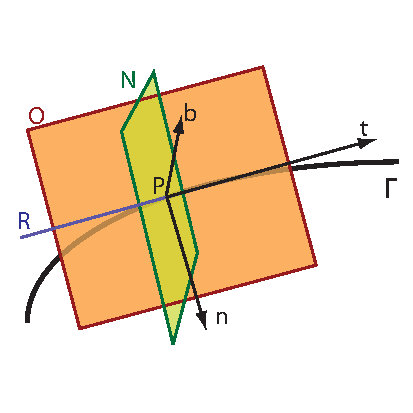
\includegraphics{Figuren/Vlakken.pdf}


\subsection{Snelheid van een Punt}
\label{sec:SnelheidPunt}
\[
  \vec{v} = \dt{\vec{r}}
          = \frac{\d{\vec{r}}}{\d{t}}
          = \frac{\d{x}}{\d{t}} \vec{1}_x + \frac{\d{y}}{\d{t}} \vec{1}_y + \frac{\d{z}}{\d{t}} \vec{1}_z
          = \dt{x} \vec{1}_x + \dt{y} \vec{1}_y + \dt{z} \vec{1}_z
\]
\[
  v       = \norm{\vec{v}}
          = \dt{s}
          = \frac{\d{s}}{\d{t}}
\]
\[
  \vec{v} = \norm{\vec{v}} \vec{1}_t
          = v \vec{1}_t
\]
\subsection{Versnelling van een Punt}
\label{sec:VersnellingPunt}
\[
  \vec{a} = \dt{\vec{v}}
          = \dtt{\vec{r}}
          = \frac{\d{^2 \vec{r}}}{\d{t^2}}
          = \frac{\d^2{x}}{\d{t^2}} \vec{1}_x + \frac{\d^2{y}}{\d{t^2}} \vec{1}_y + \frac{\d^2{z}}{\d{t^2}} \vec{1}_z
          = \dtt{x} \vec{1}_x + \dtt{y} \vec{1}_y + \dtt{z} \vec{1}_z
\]
\[
  \vec{a} = \dt{v} \vec{1}_t + \frac{v^2}{R} \vec{1}_n
          = \frac{\d{v}}{\d{t}} \vec{1}_t + \frac{v^2}{R} \vec{1}_n
          \qquad \qquad \mbox{ontbinding van Huygens}
\]
\[
  a^2    = \norm{\vec{a}}^2
         = \left( \frac{\d{v}}{\d{t}} \right)^2 + \frac{v^4}{R^2}
         = \dt{v}^2 + \frac{v^4}{R^2}
\]

\subsection{Drievlakshoek van Frenet}
\label{sec:DrievlakshoekFrenet}
\[
  \left( \vec{1}_t , \vec{1}_n , \vec{1}_b\right)
\]
\[
  \vec{1}_t \times \vec{1}_n = \vec{1}_b
\]
\[
  \vec{1}_b = \frac{\dt{\vec{r}} \times \dtt{\vec{r}}}{\norm{\dt{\vec{r}} \times \dtt{\vec{r}}}}
\]
\[
  \vec{1}_t = \frac{\dt{\vec{r}}}{\norm{\dt{\vec{r}}}}
            = \frac{\vec{v}}{\norm{\vec{v}}}
            = \frac{\dt{\vec{r}}}{\dt{s}}
            = \frac{\d{\vec{r}}}{\d{s}}
            = \ds{\vec{r}}
\]
\[
  \vec{1}_n = \vec{1}_b \times \vec{1}_t
\]

\subsection{Formules van Frenet}
\label{sec:FormulesFrenet}
\[
  \frac{\d{\vec{1}_t}}{\d{s}} = \frac{1}{R}\vec{1}_n
\]
\[
  \frac{\d{\vec{1}_b}}{\d{s}} = \frac{1}{T}\vec{1}_n
\]
\[
  \frac{\d{\vec{1}_n}}{\d{s}} = - \frac{1}{R} \vec{1}_t - \frac{1}{T} \vec{1}_b
\]

\subsection{Kromtecirkel en Kromtestraal}
\label{sec:KromtecirkelEnKromtestraal}
\[
 \rho = R = \pm \frac{\d{s}}{\d{\alpha}} > 0
\]

\paragraph{Kromtestraal met baan in parametervorm}
\label{sec:KromtestraalParametervorm}
$\Gamma : x\left(t\right), y\left(t\right)$
\[
  \rho = \pm \frac{\left(\dt{x}^2 + \dt{y}^2\right)^{3/2}}{\dt{x}\dtt{y} + \dt{y}\dtt{x}}
\]

\paragraph{Kromtestraal met baan in natuurlijke parametervorm}
\label{sec:KromtestraalNatuurlijkeParametervorm}
$\Gamma : x\left(s\right), y\left(s\right)$
\[
  \rho = \pm \frac{1}{\ds{x}\dss{y} + \ds{y}\dss{x}}
\]

\paragraph{Kromtestraal met baan als functievoorschrift}
\label{sec:KromtestraalFunctievorm}
$\Gamma : y = y\left( x \right)$
\[
  \rho = \pm \frac{\left(1 +\dx{y}^2\right)^{3/2}}{\dxx{y}} \qquad \qquad \mbox{met } \dx{} = \frac{\d{}}{\d{x}}
\]

\paragraph{Kromtestraal in 3 dimensies}
\label{sec:Kromtestraal3D}
$\Gamma : x\left(t\right), y\left(t\right), z\left(t\right)$
\[
  R = \frac{1}{\sqrt{\dss{x}^2 + \dss{y}^2 + \dss{z}^2}}
\]

\subsection{Perksnelheid en -versnelling}
\label{sec:Perksnelheid}
\[
  \vec{v}_{perk} = \frac{\d{\vec{S}}}{\d{t}} = \frac{1}{2} \vect{OP} \times \vec{v} = \frac{1}{2} \vec{M}_O (\vec{v})
\]
\[
  \vec{a}_{perk} = \frac{\d^2{\vec{S}}}{\d{t}^2} = \frac{1}{2} \vect{OP} \times \vec{a} = \frac{1}{2} \vec{M}_O (\vec{a})
\]

\subsection{Relatieve beweging}
Een index $_O$ slaat op de oorsprong van het relatief assenstelsel.
Een index $_R$ slaat op de coördinaten in het relatief assenselsel.
Let op de gebruikte assenstelsel bij het onbinden in componenten!
\[
  \vec{r} = \vec{r}_O + \vec{r}_R
\]
\[
  \vec{v} = \vec{v}_R + \vec{v}_s
\]
\[
  \vec{a} = \vec{a}_R + \vec{a}_s + \vec{a}_c
\]
Hierin zijn:
\[
  \vec{v}_s = \vec{v}_O + \vec{\omega} \times \vec{r}_R
\]
\[
  \vec{a}_s = \vec{a}_O + \dt{\vec{\omega}} \times \vec{r}_R + \vec{\omega} \times \left( \vec{\omega} \times \vec{r}_R \right)
\]
\[
  \vec{a}_c = 2 \vec{\omega} \times \vec{v}_R
\]



